\documentclass{boi2014-fi}

\usepackage{enumitem}

\renewcommand{\DayNum}{2}
\renewcommand{\TaskCode}{portals}
\renewcommand{\TaskName}{Portaalit}

\newcommand{\constant}[1]{{\tt #1}}

\begin{document}
    \begin{wrapfigure}[4]{r}{4cm}
        \vspace{-24pt}
\includegraphics[width=4cm]{\TaskCode.jpeg}
\end{wrapfigure}

    Labyrintin sisällä on kakunpala, ja haluat epätoivoisesti syödä sen.
    Sinulla on labyrintin kartta, joka on $R$ rivistä ja $C$ sarakkeesta
    muodostuva ruudukko.
    Jokaisessa ruudussa on yksi seuraavista merkeistä:

    \begin{description}[itemindent=1pt]
     \item[\constant{\#}] (risuaita) joka tarkoittaa seinää,
        \item[\constant{.}] (piste) joka tarkoittaa tyhjää ruutua,
        \item[\constant{S}] (suuri s) joka tarkoittaa tyhjää ruutua,
        joka on tämänhetkinen sijaintisi
        \item[\constant{C}] (suuri c) joka tarkoittaa tyhjää ruutua,
        jossa on kakunpala.
    \end{description}

    Voit kulkea vain tyhjiä ruutuja pitkin ja siirtyä ruudusta toiseen,
    jos niillä on yhteinen sivu. Lisäksi kartassa kuvattu suorakulmion
    muotoinen alue on ympäröity seinäruuduilla ulkopuolelta.

    Saadaksesi kakun nopeammin sinulla on käytössä portaalipyssy
    (valmistaja Aperture Science\texttrademark{}), joka toimii seuraavasti.
    Millä tahansa ajanhetkellä pyssyllä pystyy ampumaan portaalin
    yhteen neljästä mahdollisesta suunnasta: \emph{ylös}, \emph{vasemmalle},
    \emph{alas} tai \emph{oikealle}. Kun portaali ammutaan johonkin suuntaan,
    se liikkuu kyseiseen suuntaan kunnes saavuttaa ensimmäisen seinän.
    Kun täm tapahtuu, portaali kiinnittyy seinään sille puolelle,
    joka on sinun näkyvissäsi.

    Samaan aikaan voi olla olemassa enintään kaksi portaalia.
    Jos kaksi portaalia on jo sijoitettu labyrinttiin,
    toinen niistä (valintasi mukaan) poistuu välittömästi
    käyttäessäsi portaalipyssyä uudestaan.
    Jos ammut portaalin seinään kohtaan, jossa on valmiiksi portaali,
    uusi portaali korvaa edellisen (jokaisella seinän sivulla voi
    olla korkeintaan yksi portaali). Huomaa, että kaksi portaalia
    voi olla saman seinän eri puolilla.

    Kun olet sijoittanut kartalle kaksi portaalia,
    voit käyttää niitä teleportaatioon.
    Kun seisot jommankumman portaalin vieressä,
    voit kävellä sen sisään, minkä seurauksena päädyt
    tyhjään ruutuun toisen portaalin viereen.
    Tämän tekeminen vie yhtä paljon aikaa kuin liikkuminen
    ruudusta vierekkäiseen ruutuun.

    Voit olettaa, että portaalien ampuminen ei vie yhtään aikaan ja
    kahden vierekkäisen ruudun välillä liikkuminen sekä
    teleportaatio portaalien kautta vievät yhden aikayksikön.

    \Task
    Annettuna on labyrintin kartta sekä aloituskohtasi ja kakunpalan sijainti.
    Tehtäväsi on laskea pienin mahdollinen aika,
    minkä tarvitset kakunpalan saavuttamiseen.

    \Input
    Syötteen ensimmäisellä rivillä on kaksi kokonaislukua:
    kartan rivien määrä $R$ sekä kartan sarakkeiden määrä $C$.
    Seuraavat $R$ riviä kuvaavat kartan.
    Jokaisella rivillä on $C$ merkkiä: \constant{\#},
    \constant{.}, \constant{S} or \constant{C} (näiden merkitys on kerrottu ylempänä).

    Voit luottaa siihen, että merkit \constant{S} ja \constant{C}
    esiintyvät tarkalleen kerran kartassa.

    \Output
    Tulosteessa tulee olle yksi kokonaisluku: pienin mahdollinen aika,
    jossa pystyt liikkumaan kakun luokse aloituskohdastasi.

    Voit olettaa, että aloituskohdastasi on aina mahdollista päästä kakun luokse.

    \Example
    \example
    {
        4 4\newline
        .\#.C\newline
        .\#.\#\newline
        ....\newline
        S...
    }
    {
        4
    }
    {
        Yksi nopein reitti on seuraava: 1) liiku oikealle,
        2) liiku oikealle, ammu yksi portaali ylös ja toinen portaali alas,
        3) mene alempaan portaaliin,
        4) liiku askel oikealle, jolloin saat kakun.

        \begin{center}
            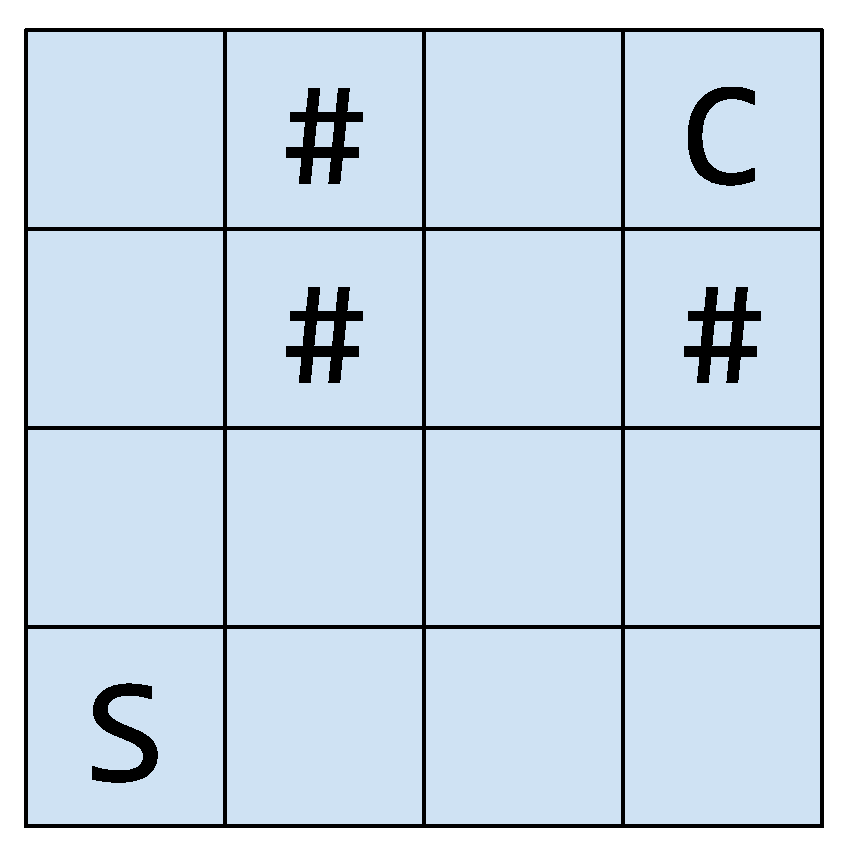
\includegraphics[width=4cm]{portals-example}
        \end{center}
    }

    \Scoring

    \begin{description}[leftmargin=0pt]
        \item[Osatehtävä 1 (? pistettä):] $0 \le R \le 10, 0 \le C \le 10$.
        \item[Osatehtävä 2 (? pistettä):] $0 \le R \le 50, 0 \le C \le 50$.
        \item[Osatehtävä 3 (? pistettä):] $0 \le R \le 200, 0 \le C \le 200$.
        Jokaisessa tyhjässä ruudussa on vähintään yksi seinä sen vieressä.
        \item[Osatehtävä 4 (? pistettä):] $0 \le R \le 200, 0 \le C \le 200$.
        \item[Osatehtävä 5 (? pistettä):] $0 \le R \le 1000, 0 \le C \le 1000$.
    \end{description}

    \Constraints

    \begin{description}
        \item[Aikaraja:] ? s.
        \item[Muistiraja:] ? MB.
    \end{description}
\end{document}